\chapter{Background}\label{ch:background}

This chapter discusses the background to this thesis.
Its aim is to give context to the project that is implemented in addition to specific technical knowledge.
The context of this work is mostly DevOps as it heavily uses implementations of DevOps practices, such as CI/CD tools which are explained in Section~\ref{sec:devops-and-agile-programming}.
Testing as a concept exists in software engineering since the beginning and deeper insights are given in Section~\ref{sec:testing}.
The DTF, briefly mentioned in Chapter~\ref{ch:introduction} implements theoretical concepts of similarity-based variability testing, which is picked up on in Section~\ref{sec:similarities}.
Finally, virtualization of applications and a technology building on top of it, Kubernetes, are described in Sections~\ref{sec:virtualization} and~\ref{sec:kubernetes}.

\section{DevOps and agile programming}\label{sec:devops-and-agile-programming}

In agile programming, different practices have emerged since the agile manifesto~\cite{AgileManifesto} appeared in 2001.
Extreme programming, Scrum and Kanban are only a few examples of such practices~\cite{ADecadeOfAgileMethodologies}, all of them aim at increasing the velocity of software development and the speed at which a project can change into different directions.
These agile practices are more and more adopted in the industry~\cite{BecomingAgileTogether} and taught at universities~\cite{StudienhandbuchProjectManagement}.

As an example of agile programming, Scrum can be dissected.
The inventors of Scrum, Jeff Sutherland and Ken Schwaber, describe Scrum as follows.
``Scrum is a lightweight framework that helps people, teams and organizations generate value through adaptive solutions for complex problems''~\cite{the-scrum-guide}

\pagebreak

It is meant to be simple, as well as easy to understand and execute.
According to the Scrum guide~\cite{the-scrum-guide}, it is supposed to allow changes to a system as early as possible, planning only as much as needed, and even if planned, allowing space for deviation.
In short, the goal is to have a system that allows focused planning while also having a high velocity when developing projects.

In that context, DevOps can be seen as an extension as well as an evolution of agile practices.
Instead of applying it to software development itself, it is applied to things surrounding it.
Scrum, for example, describes how a feature is supposed to be planned and implemented.
A DevOps practice describes how this feature can be integrated into the code base, tested, or distributed.

In more elaborate terms, DevOps is all about making sure new code works well and as intended~\cite{the-software-architext-and-devops}.
If code fulfills these criteria, it is supposed to be automatically integrated into the existing code base.
After the integration was successful, it should then be distributed, again automatically.
Some systems depend on certain infrastructure, such as servers.
Naturally, this infrastructure has the potential to fail.
To mitigate this, the final DevOps practice is to ensure a stable, possibly self-repairing, infrastructure~\cite{container-and-microservice-driven-design-for-cloud-infrastructure-devops}.

This thesis concerns itself with the first two principles of DevOps.
Making sure stuff works and making sure said stuff is distributed reliably.
In order to make sure stuff works and is distributed, in an automated manner, Concourse~\cite{concourse} is used.

Concourse~\cite{concourse} is a CI/CD system that can be used to automate certain development tasks and group them into a pipeline.
Tasks can then be run either concurrently or sequentially in the context of the pipeline they are grouped in.
In addition, resources to be used can be defined and added to tasks, so they are available to them.
Such resources can be files, online resources, storage locations or any number of information a task may need.
Files that are used to configure Concourse are written in either the JSON or YAML data format.

\pagebreak

From its description, it becomes clear why Concourse, or CI/CD systems in general, are heavily utilized by DevOps.
It is described as ``an open-source continuous thinger-doer''~\cite{concourse}.
Using appropriate configuration files, it can continuously and automatically do things, such as testing code, and distributing the resulting system.
Many other CI/CD systems exist as well, notably Jenkins\footnote{https://www.jenkins.io/}, GitLab\footnote{https://about.gitlab.com/}, or circleci\footnote{https://circleci.com/}.
They function in a similar manner to Concourse and could be used instead in other projects as needed.

\section{Testing}\label{sec:testing}

Arguably, if there is the need to automatically integrate code into code bases, there is also the need for testing.
After all, faulty code or code with unintended behaviour must not be integrated and certainly not automatically.
The need for automated testing is even higher if the integration task is also automated.
If code is integrated manually, a developer can also manually test its integration.
If code is integrated automatically, this might not be possible anymore.

Testing code in an automated fashion has developed as software projects grew in size and importance.
The first commercially successful programming language, Fortran, was released in 1957~\cite{history-of-software}.
In 1961, automatic testing was already in use~\cite{automatic-grading-of-graphical-user-interface-programs}.
The first documented software lifecycle model, the waterfall model, was documented in 1970~\cite{history-of-waterfall-model}.
This very first model already includes testing as part of its lifecycle.

\begin{figure}[h]
    \centering
    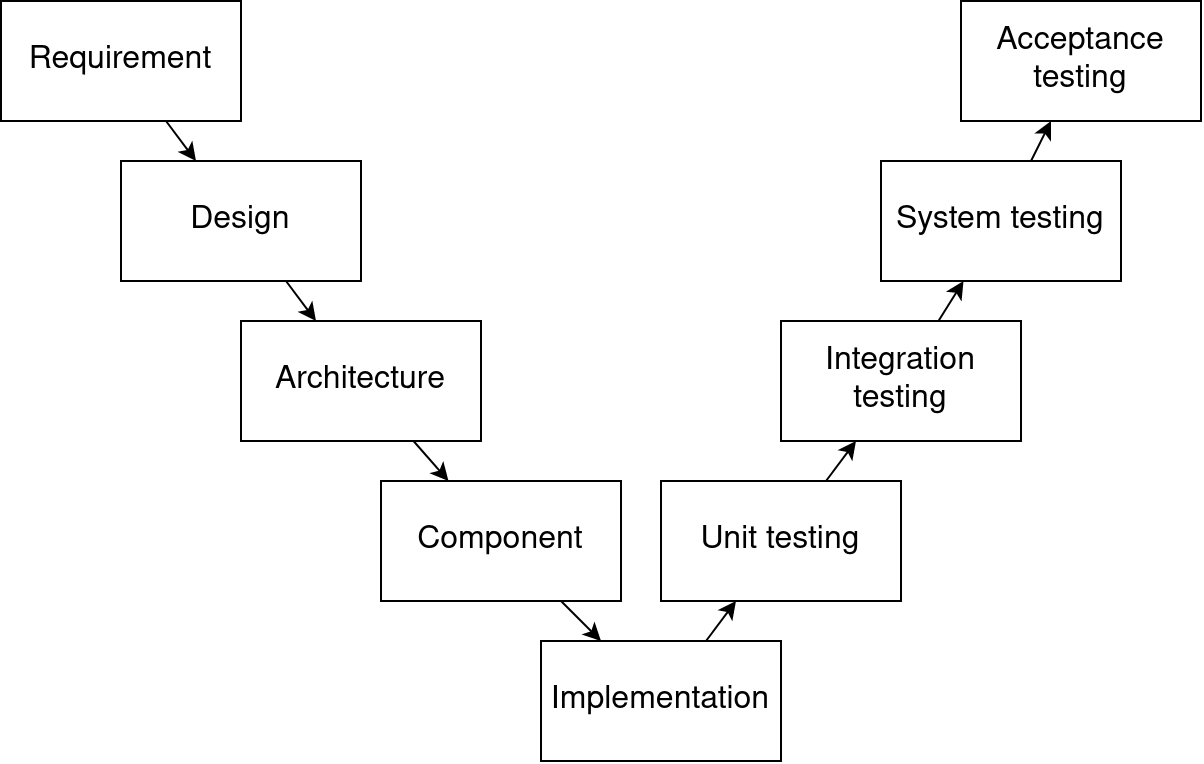
\includegraphics[width=0.5\textheight]{img/introduction/software-testing-v.drawio}
    \caption{Levels of abstraction and their corresponding tests~\cite{waterfall-vs-v-model-vs-agile}.}
    \label{fig:levels-of-abstraction-and-tests}
\end{figure}

Figure~\ref{fig:levels-of-abstraction-and-tests} describes another model, the V-model~\cite{waterfall-vs-v-model-vs-agile}.
Although in general it is considered out of date for many development contexts, given that agile practices are used nowadays as described before, it is helpful to visualize the layers of systems and their corresponding tests.
Single components are unit tested in isolation, while their interaction is tested using integration tests and so on and so forth.
In order to validate code before an automatic integration occurs, a well-founded set of tests is needed.
Not only on the lowest levels, but also on the highest level, which is acceptance testing.
Without strong test suits, faulty code may be integrated into a system and then delivered to stakeholders.

This thesis focuses on the second layer of testing, i.e., integration testing.
Integration testing commonly take the form of \textbf{End-to-End (E2E) testing}~\cite{end-to-end-integration-testing-design}.
As the name suggests, this technique tests a software system from one end, i.e., a hypothetical user, across user-system interaction, to the other end, i.e., the results of a feature.

For example, buying an item on an online shop can be tested using e2e tests.
First, a test program may open a browser and navigate to the website.
It then adds certain items to a cart, evaluating the shown total on the site.
It then removes and re-adds certain items while evaluating the subtotal.
After the purchase is completed, it checks that the correct entries where made in the datastore of the web shop and that all transactions were made correctly and completely.

\section{Virtualization}\label{sec:virtualization}

Some of the implementation part of this thesis is build upon Kubernetes, which is discussed in Section~\ref{sec:kubernetes}.
However, to effectively explain what Kubernetes is and does, containerization must first be explained.
Containerization on the other hand is a subcategory of the more general field of virtualization.

\begin{figure}[H]
    \centering
    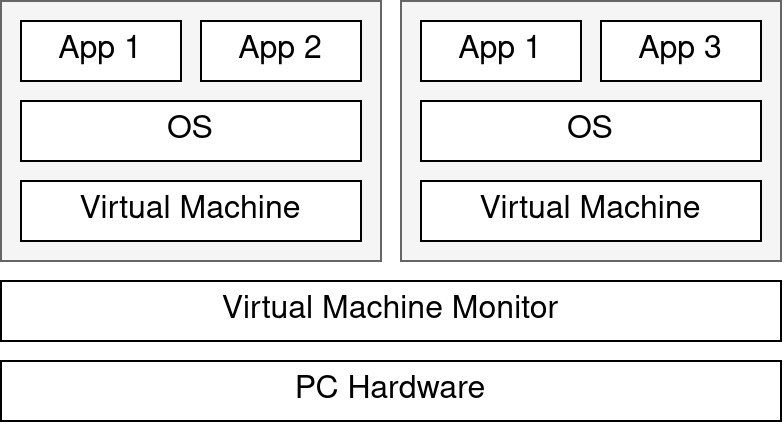
\includegraphics[width=0.5\textwidth]{img/background/standalone-vm}
    \caption{Standalone VM~\cite{a-survey-on-virtualization-technologies}.}
    \label{fig:standalone-vm}
\end{figure}

\begin{figure}[H]
    \centering
    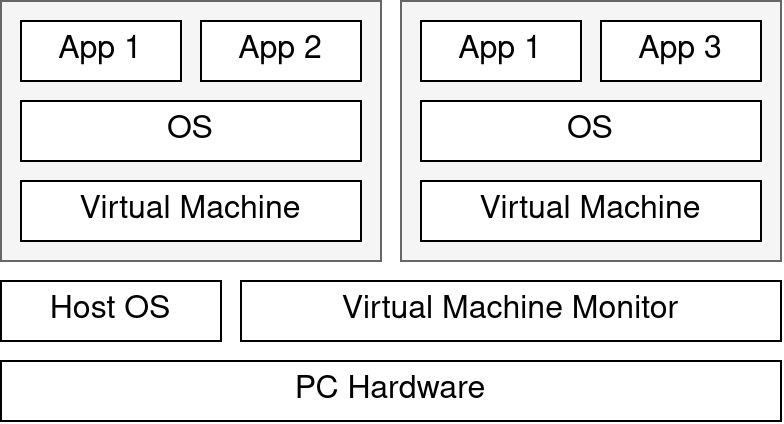
\includegraphics[width=0.5\textwidth]{img/background/hosted-vm}
    \caption{Hosted VM~\cite{a-survey-on-virtualization-technologies}.}
    \label{fig:hosted-vm}
\end{figure}


There are three types of virtualization that are commonly used nowadays~\cite{containers-vs-virtual-machines, a-survey-on-virtualization-technologies}.
First, virtualization using a virtual machine (VM) that utilizes the host's hardware, also called a Standalone Virtual Machine seen in Figure~\ref{fig:standalone-vm}.
Second, virtualization using a VM that runs on top of a host operating system, plainly called Hosted Virtual Machine seen in Figure~\ref{fig:hosted-vm}.
Both utilize techniques to run a full OS, sandboxed as a process, either on a host or shared hardware.

\begin{figure}[H]
    \centering
    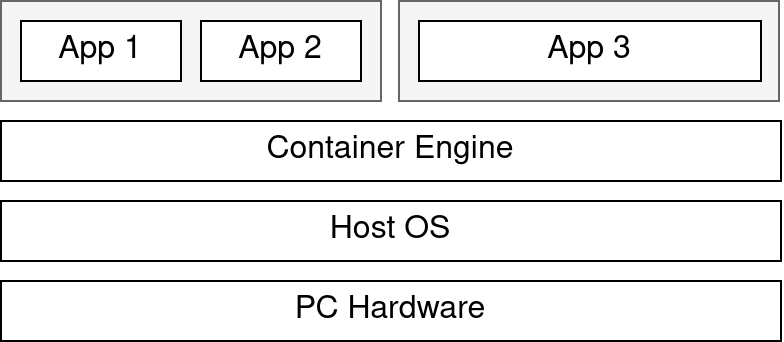
\includegraphics[width=0.5\textwidth]{img/background/container}
    \caption{Containerization.}
    \label{fig:containerization}
\end{figure}

A container~\cite{what-are-linux-containers} is a process that runs on an operating system (OS), which is mostly isolated from the host system and other processes that run on it.
In a way, they act as virtual machines.
However, they do not contain an OS themselves, but make use of the host OS through abstraction layers as seen in figure~\ref{fig:containerization}.
The advantage of not having to virtualize the OS is usually a better performance compared to virtual machines.
On the other hand, due to them not being completely isolated from the host OS, they have a larger impact on a system's security.

\section{Kubernetes}\label{sec:kubernetes}

A large part of this thesis concerns itself with a technology called \textbf{Kubernetes}.
Kubernetes is a complex software system and care must be taken to establish different parts and concepts of it.
This section covers the basic information needed to understand how it works and what certain terminology means in its context.

First, \textbf{Images} and \textbf{Containers}~\cite{docker-image,kubernetes-images,kubernetes-containers} act as the base of Kubernetes.
An image can be seen as a template including instructions to create a container.
These instructions can range from simple commands to complex, multistep build instructions.
Any image can also serve as the starting point for a new image.
This allows the creation of complex systems that can be instantiated as containers at any time.

A Kubernetes system is structured as a \textbf{cluster} and therefore called a ``Kubernetes cluster''~\cite{kubernetes-cluster}.
It is called a cluster because it is made of a cluster of \textbf{nodes}.
In the context of Kubernetes, a node is a computer that serves as a part of a cluster.

The smallest clusters typically have three nodes~\cite{kubernetes-cluster}, one control node and multiple worker nodes.
It is possible to have clusters with only one or two nodes, but they are mostly only used for development and debugging purposes~\cite{minikube}.
Bigger clusters and clusters that are made for software systems with high availability requirements can also have multiple control nodes for redundancy.
In such a cluster, worker nodes interact with one control node at a time, with other control nodes taking over if one fails.

\pagebreak

\textbf{Pods}~\cite{kubernetes-pods} are the smallest units of work a Kubernetes cluster uses to handle workloads.
A pod can consist of multiples containers and groups them logically.
When deploying a container that way, a pod can manage the environment of the pod, such as mounted directories, network capabilities or environment variables.
Furthermore, a pod can have three different kinds of containers, normal containers, \textbf{init-containers} and ephemeral containers.
Normal containers describe the main workload of the pod.
Usually the main application is run inside one container, while other tasks, such as logging, is done in another.
This pattern is called Sidecar pattern and such pods are commonly referred to as \textbf{sidecar containers}~\cite{sidecar-container}.
These containers are only started, however, after all of a pods init-containers have succeeded.
For example, a pod may have a web server as a container that it runs continuously, but has an init container that executes setup tasks that need to run before the server starts.
Finally, ephemeral containers are containers added to an already deployed pod to be used for debugging.

\textbf{ReplicaSets}~\cite{kubernetes-replicaset} are the simplest form of deploying multiple instances of pods.
They are defined by providing a template of a pod and the number of replicas of the given template.
The replicaset then does its best to deploy the specified amount of pods on the cluster.
It schedules new ones if there are too few and deletes pods if there are too many.
However, sometimes it is not possible for a specific amount of pods to actually be deployed due to resource constraints of the cluster and its nodes.

\textbf{Deployments}~\cite{kubernetes-deployments} build on top of replica sets.
They are also defined by a pod specification and the required amount of replicas.
However, a deployment does not manage the pods, but uses a replica set to do so.
This enables a deployment to, for example, do rolling updates ``automagically''\footnote{Automatically, but being reminiscent of wizardry}.
When a deployment is changed, it can decrease the desired amount of replicas of the original replicaset, while gradually increasing it for the new one.
An application can be updated seemingly and gradually to a new version, to avoid service outages in case of bugs or server downtimes.

Similar to deployments, \textbf{StatefulSets}~\cite{kubernetes-statefulsets} handle the deployment of pods.
The difference is, that the name, i.e., the identity, of a pod is guaranteed.
When a pod is created through a replica set or a deployment, the pod is assigned a semi-random name consisting of the deployment or replicaset name and random string.

A pod created by a stateful set on the other hand is usually named with the name of the stateful set with the index of the pod at the end.
For example, a pod of a deployment with the name of ``my-app'' results in the pod being named ``my-app-asd123-fgh456''.
A pod of a stateful set of the same name would result in the name being ``my-app-1''.
Furthermore, the naming is made consistent.
If a stateful set controls three pods, ``pod-1'', ``pod-2'', and ``pod-3'', and ``pod-2'' is deleted, it will try to deploy a new pod with the name ``pod-2''.

The \textbf{Kubernetes API}~\cite{kubernetes-api} is the part of Kubernetes that receives resource requests, i.e., if an administrator wants to create resource, such as a pod, a HTTP request is sent to the Kubernetes API describing that resource.
From there, it is then applied to the cluster and other Kubernetes components are notified.
Interacting with this API is commonly abstracted to the Kubernetes CLI for manual, or client libraries for automatic communication.

\textbf{Webhooks}~\cite{kubernetes-webhooks} are used to catch requests for pods and modify them before they are scheduled.
Whenever a resource is modified in a cluster, it is handled as a HTTP request.
These HTTP requests can then be sent to a webhook, before they are returned to Kubernetes for further processing.
Webhooks that are used to mutate a resource are called mutating admission webhooks.
A different type of webhook also exists called validating admission webhook.
This type of webhook does not mutate a resource but is used to either allow or deny a resource being modified.

\textbf{Manifests}~\cite{kubernetes-manifests} represent the state of a Kubernetes cluster as a configuration file.
These configuration files are written in YAML.
When such a configuration is applied to a cluster, Kubernetes tries to create the state that is described by this configuration.
Multiple resources can be defined in a single configuration.
Multiple configurations can be applied to a single cluster.
Note well that these files are static, meaning that they do not accept the application of variables when applied to Kubernetes.

In order to manipulate manifests dynamically \textbf{Helm charts}~\cite{helm-charts} can be used.
A Helm chart is a package containing templates of Kubernetes resources and metadata.
Helm charts also include a way to configure these templates.
When a Helm chart is applied to a Kubernetes cluster, this configuration can be changed, either manually or dynamically.
The resources are then generated based on the supplied configuration.
Helm charts can also be compiled to an archive and distributed as such or as part of a repository.

\pagebreak

\textbf{Operators}~\cite{kubernetes-operator} are custom systems that interact with the Kubernetes API from within a Kubernetes cluster.
To do so, they often supply their own custom resource with which an administrator can configure an operator.
An operator's functionality is custom, but it is commonly deploying other resources on demand or maintaining them.
As previously mentioned, Kubernetes manifests are usually static, but an operator can be used to configure these resources on the line.

The \textbf{Operator Framework}~\cite{operator-framework, operator-lifecycle-manager} is a set of libraries which makes it easier to create operators in the Golang language.
In combination with the \textbf{Operator Lifecycle Manager (OLM)}~\cite{operator-lifecycle-manager}, operators created with this framework can be more easily run in a range of clusters.
OLM describes and handles how an operator can be installed and managed on a cluster.
Providers that offer Kubernetes clusters as a service can include support for OLM.
These providers than commonly offer a marketplace from which an operator can be installed.

\textbf{Amazon Web Services (AWS) and GCS (Google Cloud Service)}~\cite{eks,gke} are two of the many providers of Kubernetes cluster that exists.
These two are important for this thesis, as mainly their infrastructure is used.
The specific products that are used to create a cluster are called Elastic Kubernetes Service (EKS) and Google Kubernetes Engine (GKE) respectively.
EKS is later used to create clusters that run Openshift.

\textbf{Openshift}~\cite{openshift} is a software system built on top of a Kubernetes cluster.
It abstracts different aspects of cluster administration, such as resource or credential management.
Furthermore, it provides a marketplace from RedHat that uses OLM to install and manage operators.


\section{Similarity-based variability testing}\label{sec:similarities}

As previously discussed, one of the main difficulties of testing highly scaled and complex systems, is the need of setting up complex environments.
Later it is shown, that for certain technologies, the setup for a single test may take multiple hours.
For large test suites, it is therefore unpractical to run all tests every time, as the time-cost would be too high.
In order to mitigate this issue, a technique called similarity-based variability testing is used.

Al-Hajjaji et al.~describe this technique in the context of product line testing~\cite{SimilarityBasedPrioritizationInSoftwareProductLineTesting}.
A software product line is described as a base software system, which is extended with features that make use of the base system.
Due to the high variability, not all combinations and features can be practically tested.
Therefore, an algorithm is proposed, that selects tests based on similarity.

This algorithm uses a set of possible configurations, \textit{C} and a predefined definition of their similarity \textit{S} to each other\footnote{The used variable names C and S do not correspond to the variable names in the original algorithm.}.
For example, given mobile phones, two phones that both integrate a GPS transceiver are more similar to each other, than one phone that does and one that does not.
It then takes the first configuration from the input set and adds it to the result.
Then, from the selected configuration, the next, least similar, configuration is selected.
This selection is added to the result and the next, least similar, configuration to this second one is chosen.
The algorithm then continues until all configurations are sorted in the result or a limit is reached.

This algorithm, while used in a different context, is also valuable when testing complex system.
As previous discussed, for sufficiently complex environments and large test suites, not all tests can realistically be run at all times.
Analogous to configurations, metadata can also be added to define the similarity of tests to each other.
A similar algorithm as described above can then be used to sort and select tests which are possible to run in a limited timeframe.
In Section~\ref{sec:dynamic-testing-framework} it is shown that this algorithm helps in implementing a solution for the problem of abstracting pipeline configurations.

\section{Other technologies and concepts}\label{sec:technologies-used}

There are also a handful of other technologies and concepts used in this work not previously mentioned.
They are simple enough to not warrant whole sections dedicated to them.
Therefore, they are listed here and shortly summarized.
The name and, if applicable, the acronym of a technology is stated followed by a short description of it.

\pagebreak

\textbf{BitBucket}~\cite{bitbucket} is a system that utilizes \textbf{Git}~\cite{git} to store project files.
Git is used to version a project and make it easier for a team of people to simultaneously work on a project.
A project that is worked on in this manner is commonly called a repository.
BitBucket itself then stores the repository online to ease access to it.

\textbf{Vault}~\cite{vault} is a system created by HashiCorp to manage credentials.
It offers a user interface as well as a backend to store secrets, en- and decrypt them as wells as user management.
The backend is accessible either through the provided client or the provided API.
This API is used by Concourse to retrieve secrets during pipeline runs.

\textbf{Permission bits}~\cite{unix-file-permissions} are used by unix file systems to control access to files.
Each file has three groups with three bits each.
Every bit signifies if a certain action, reading, writing, or executing, can be taken for a file.
The groups determine what the file owner, a group member or any other user, can do.
For example:

A file's permission bits are set to $7$, $4$, and $2$, or $742$ as a shorthand notation.
Note here that $742$ does not represent the number sevenhundredfortytwo, but the decimal value of each group as a shortened form.
That means, the file owner can do everything with the file, because the number $7$ in binary is represented as $111$.
Therefore, all permission bits are set.
Next, the number $4$ represents what the group of users that owns the file can do.
A $4$ in binary is represented as $100$.
That means, members of the group may read the file, but may neither write nor execute it.
Finally, the $2$ represents what every user in the system can do.
Since $2$ is represented as $010$, the permission bit for writing a file is set.
So every user, that is neither the file owner nor a member of the aforementioned group, may write a file, but neither read nor execute it.

\textbf{Representational State Transfer}~\cite{extending-representation-state-transfer} is a way to build decentralized systems which depend on sharing resources.
A REST based system commonly builds on top of HTTP to request, process and transmit resources.
Commonly, a REST server is stateless, i.e., the server is not aware of any state when a request is processed.

